% Use only LaTeX2e, calling the article.cls class and 12-point type.

\documentclass[12pt]{article}

% Users of the {thebibliography} environment or BibTeX should use the
% scicite.sty package, downloadable from *Science* at
% www.sciencemag.org/about/authors/prep/TeX_help/ .
% This package should properly format in-text
% reference calls and reference-list numbers.

\usepackage{scicite}

% Use times if you have the font installed; otherwise, comment out the
% following line.

\usepackage{times}

\usepackage{graphicx}

% The preamble here sets up a lot of new/revised commands and
% environments.  It's annoying, but please do *not* try to strip these
% out into a separate .sty file (which could lead to the loss of some
% information when we convert the file to other formats).  Instead, keep
% them in the preamble of your main LaTeX source file.


% The following parameters seem to provide a reasonable page setup.

\topmargin 0.0cm
\oddsidemargin 0.2cm
\textwidth 16cm 
\textheight 21cm
\footskip 1.0cm


%The next command sets up an environment for the abstract to your paper.

\newenvironment{sciabstract}{%
\begin{quote} \bf}
{\end{quote}}


% If your reference list includes text notes as well as references,
% include the following line; otherwise, comment it out.

\renewcommand\refname{Literaturverzeichnis}

% The following lines set up an environment for the last note in the
% reference list, which commonly includes acknowledgments of funding,
% help, etc.  It's intended for users of BibTeX or the {thebibliography}
% environment.  Users who are hand-coding their references at the end
% using a list environment such as {enumerate} can simply add another
% item at the end, and it will be numbered automatically.

\newcounter{lastnote}
\newenvironment{scilastnote}{%
\setcounter{lastnote}{\value{enumiv}}%
\addtocounter{lastnote}{+1}%
\begin{list}%
{\arabic{lastnote}.}
{\setlength{\leftmargin}{.22in}}
{\setlength{\labelsep}{.5em}}}
{\end{list}}


% Include your paper's title here

\title{Clustern von Eye-Trackingdaten zur Unterstützung bei der Früherkennung von Dyslexie} 


% Place the author information here.  Please hand-code the contact
% information and notecalls; do *not* use \footnote commands.  Let the
% author contact information appear immediately below the author names
% as shown.  We would also prefer that you don't change the type-size
% settings shown here.

\author
{Mario Kaulmann,$^{1}$ Herval Nganya,$^{1}$\\
\\
\normalsize{$^{1}$University of Applied Sciences, Technische Hochschule Brandenburg,}\\
\normalsize{Magdeburger Stra\ss{}e 50, 14770 Brandenburg an der Havel, Deutschland}\\
}

% Include the date command, but leave its argument blank.

\date{}



%%%%%%%%%%%%%%%%% END OF PREAMBLE %%%%%%%%%%%%%%%%



\begin{document} 

% 1,5 fach Zeilenabstand

\baselineskip18pt

% Make the title.

\maketitle 



% Place your abstract within the special {sciabstract} environment.

\begin{sciabstract}
  In dieser Arbeit werden Versuchspersonen mittels Eye-Trackingdaten geclustert. Diese Versuchspersonen sollten bei der Datenerfassung drei Versuche nacheinander durchf\"uhren. Bei diesen Versuchen sollte ein Punkt mit dem Blick verfolgt werden. Bei der Clusterung soll sich herausbilden, wie gut die Versuchspersonen diese Aufgabe gel\"ost haben. Die Bemessung der G\"ute der Cluster erfolgt mit Hilfe des Silhouettenkoeffizienten.
\end{sciabstract}



% In setting up this template for *Science* papers, we've used both
% the \section* command and the \paragraph* command for topical
% divisions.  Which you use will of course depend on the type of paper
% you're writing.  Review Articles tend to have displayed headings, for
% which \section* is more appropriate; Research Articles, when they have
% formal topical divisions at all, tend to signal them with bold text
% that runs into the paragraph, for which \paragraph* is the right
% choice.  Either way, use the asterisk (*) modifier, as shown, to
% suppress numbering.

\section*{Einf\"uhrung}

In einem Experiment wurden Eyetracking-Daten erhoben, bei denen die Versuchspersonen drei verschiedene Versuche durchf\"uhren sollten. Dabei sollten die Versuchspersonen mit den Augen einem Punkt folgen, der eine spezielle Figur zeichnete. Diese Figuren sind eine liegende Acht und eine horizontale Linie. F\"ur jeden Versuch wurden zwei Durchl\"aufe gemacht. Pro Durchlauf wurde die entsprechende Figur zwei mal gezeichnet. F\"ur die liegende Acht langsam wurde zus\"atzlich vorher ein Probedurchlauf gemacht, bei dem die Figur nur einmal gezeichnet wurde.
Die Tabelle \ref{tab:Versuche} zeigt die Versuche, die durchgef\"uhrt wurden.\\
Die Versuchspersonen sollen so geclustert werden, dass die entstehenden Cluster zur Klassifizierung neuer Daten genutzt werden k\"onnen. Diese Cluster sollen durch eine transparente Darstellung zur Entscheidungsfindung beitragen, ob ein Kind an Dyslexie leidet.

\begin{table}[h]
	\caption{\label{tab:Versuche}Liste der Versuche: Hier wird die Reihenfolge der Versuche angegeben, sowie die Figur, die der Punkt ge\-zeich\-net hat und die Dauer eines Durchlaufs.}
	\noindent \centering{}
	\bgroup
	\def\arraystretch{2}  %  1 ist der Standardwert
	\begin{tabular}{|l|l|l|}
		\hline
		\textbf{Reihenfolge} & \textbf{Figur} & \textbf{Dauer}\\
		\hline \hline
		1 & liegende Acht langsam & 8 Sekunden\\
		\hline
		2 & liegende Acht schnell & 4 Sekunden\\
		\hline
		3 & horizontale Linie & 4 Sekunden\\
		\hline
	\end{tabular}
	\egroup
\end{table}

\section*{Daten}
Die erhobenen Eye-Trackingdaten sind Zeitreihen. Zu 302 Versuchsperson gibt es je eine Datei mit den Blickpunktdaten der Person und eine Datei mit den Koordinaten des Punkts, der verfolgt werden sollte.
Mittels dieser Zeitreihen werden personenbezogene Merkmale erzeugt, die zur Clusterung der Versuchspersonen genutzt werden k\"onnen.
Abbildung \ref{fig:rohdaten} zeigt, die Rohdaten einer Durchführung der liegenden Acht. Daraus wird deutlich, dass die Koordinatensysteme zueinander verschoben sind. Die Verschiebung betr\"agt 640 px in X-Richtung und 512 px in Y-Richtung.

\begin{figure}[h]
	\noindent \begin{centering}
		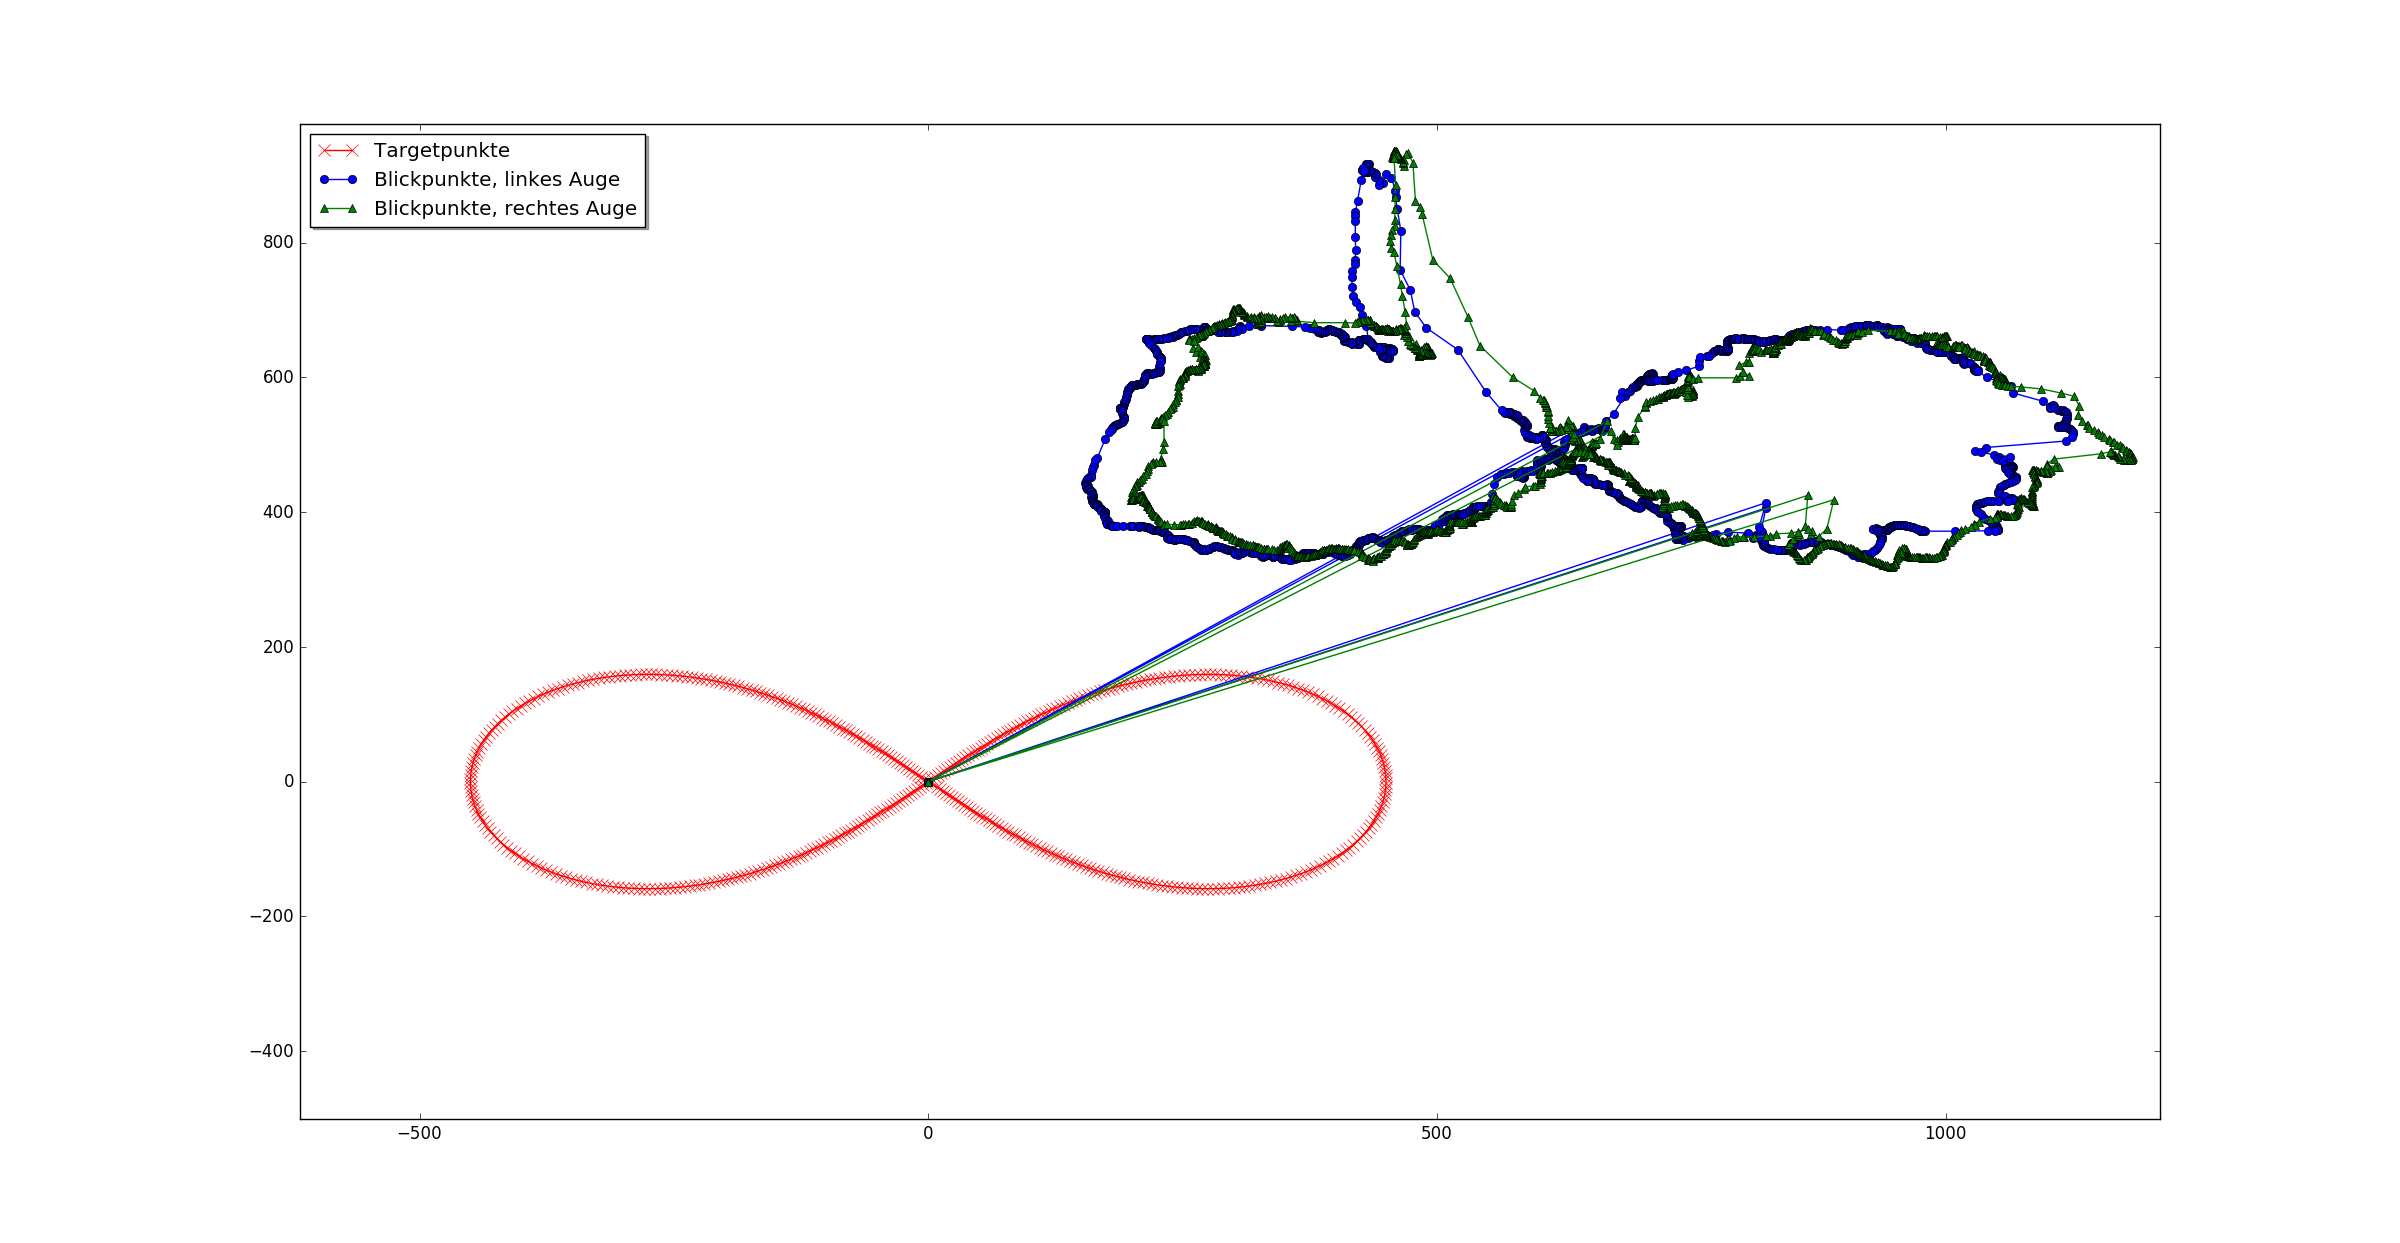
\includegraphics[width=17cm]{Bilder/bspRohdaten.png}
		\par\end{centering}
	\caption{\label{fig:rohdaten}Beispiel liegende Acht: in rot sieht man die aufgezeichneten Zielpunkte, in blau die aufgezeichneten Punkte der Blickpositionen des linken Auges und in gr\"un die Blickpositionen des rechten Auges.}
\end{figure}

\section*{Methoden}
Das Vorgehen untergliedert sich in vier Phasen. Die erste ist die explorative Analyse. Dabei werden die Daten auf Besonderheiten und ihre Wertebereiche untersucht. Die zweite Phase ist die Merkmalsgenerierung, dabei werden aus den Zeitreihen Merkmale zur Beschreibung der Versuchspersonen generiert. In der dritten Phase werden die Cluster erstellt und die G\"ute mittels Silhouettenkoeffizient bestimmt. In der vierten Phase wird ein transparentes Modell zur Beschreibung der Cluster erstellt.

\bibliography{quellen}

\bibliographystyle{apalike}

\end{document}




















